\chapter{Численные эксперименты}\label{chap2}


%%%%%%%%%%%%%%%%%%%%%%%%%%%%%%%%%%%%%%%%%%%%%%%%%%%%%%%%%%%%%%%%%%%%%%%%%%%%%%%%
\section{Применение параметрического программирования в задаче синтеза оптимальной линейной системы}\label{2sec:parametric-programming}
%%%%%%%%%%%%%%%%%%%%%%%%%%%%%%%%%%%%%%%%%%%%%%%%%%%%%%%%%%%%%%%%%%%%%%%%%%%%%%%%
Для реализации решения задачи используется MPT3 Toolbox для Matlab, описанный в главе выше.

Первоначально нужно задать все начальные значения, чтобы передать их в $mpt constructMatrices$.
$Mpt constructMatrices$ представляет собой функцию, на вход которой приходят параметры $probStruc$t и $sysStruct$.
sysStruct будет состоять из матриц A, B, C, D, ограничений на $x$ ($x_min$ и $x_max$) и ограничений на $u$ ($u_min$ и $u_max$).
$probStruct$ в свою очередь будет состоять из нормы (norm), числа N, также Q,$P_n$,R и тд.
\begin{verbatim}
N = 20;
tf = 10;
A = [0 1; -1 0];
B = [0; 1];
eps = 0.1;

sys = ss(A, B, [], []);

sysd = c2d(sys,tf/N,'zoh');
Ad = sysd.A;
Bd = sysd.B;

sysStruct.A= Ad;
sysStruct.B= Bd;
sysStruct.C= [0 0];
sysStruct.D= 0;

sysStruct.xmin = [-10; -10];
sysStruct.xmax = [10; 10];

sysStruct.umin = -1;
sysStruct.umax = 1;

nx = size(A, 2); 
probStruct.norm=inf;
probStruct.Q=[0 0; 0 0];
probStruct.P_N=[0 0; 0 0];
probStruct.R=1;
probStruct.N=N;
probStruct.subopt_lev=0;
H = [eye(nx); -eye(nx)];
K = eps*ones(nx*2,1);
probStruct.Tconstraint=2;
probStruct.Tset = polytope(H, K);
\end{verbatim}
Далее нужно на основании $mpt constructMatrices$ посмотрить класс Opt, который инкапсулирует информацию и решения для задач LP/QP/pLP/pQP/LCP/pLCP.
Для конкретного момента времени высчитаывается u на основании заданного $x_\tau$ и подается на систему. Затем на каждом отрезке из T пересчитвается заданное $x_\tau$.

\begin{verbatim}
for tau = 0:NN-1
    probStruct.N=N;
    Matrices = mpt_constructMatrices(sysStruct,probStruct);
    plp = Opt(Matrices);
    solution = plp.solve();
    u = solution.xopt.feval(xtau, 'primal');
    if N > NN/2
        xtau = Ad * xtau + Bd * u(1) + w;
    else
        xtau = Ad * xtau + Bd * u(1);
    end
    
    figure;
    solution.xopt.fplot('obj');
    xlabel('x0');
    ylabel('J(x0)');
    N = N-1;
    X = [X xtau];
    U = [U u(1)];
end
\end{verbatim}
\bigskip


%%%%%%%%%%%%%%%%%%%%%%%%%%%%%%%%%%%%%%%%%%%%%%%%%%%%%%%%%%%%%%%%%%%%%%%%%%%%%%%%
\section{Результаты}\label{2sec:results}
%%%%%%%%%%%%%%%%%%%%%%%%%%%%%%%%%%%%%%%%%%%%%%%%%%%%%%%%%%%%%%%%%%%%%%%%%%%%%%%%
Далее проилюстриуем наглядно полученные результаты на каждом 5 шаге\\ 

N = 20
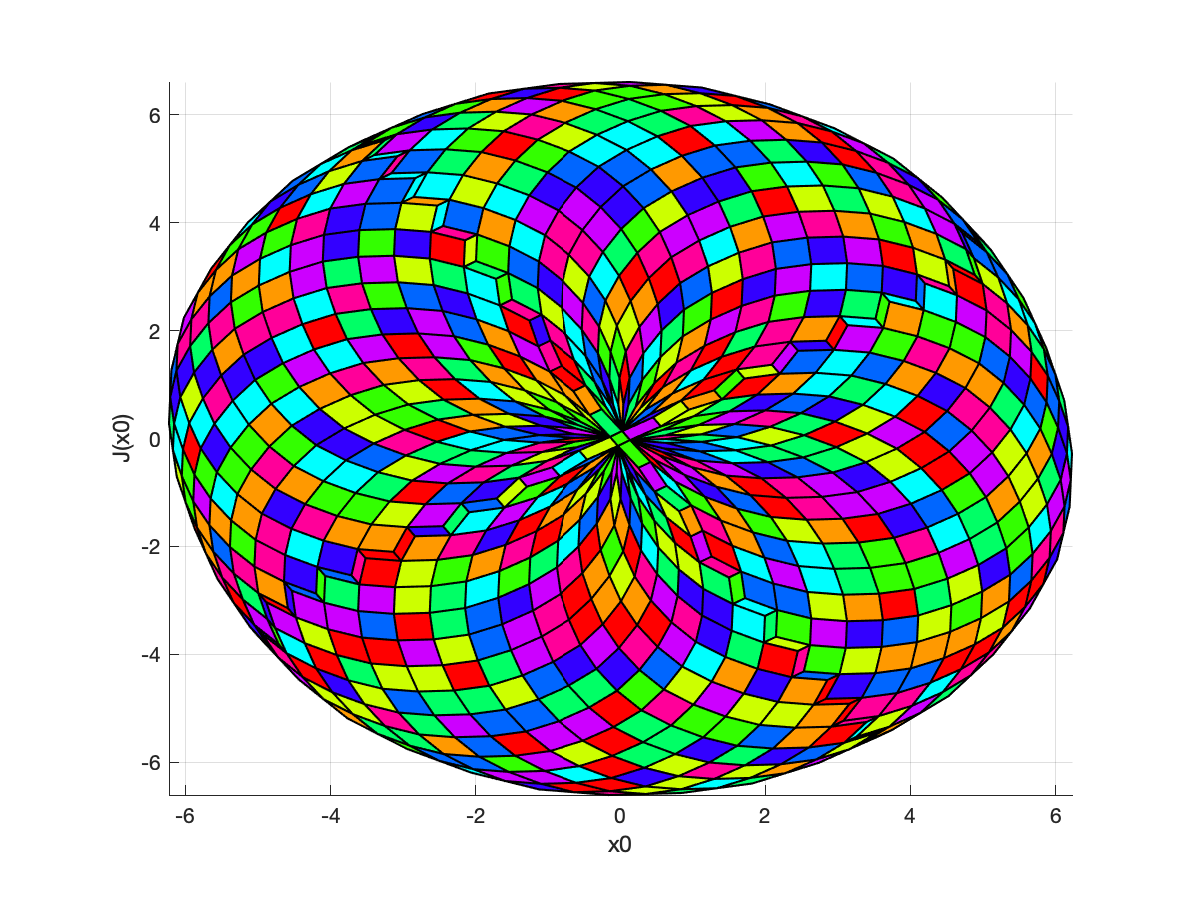
\includegraphics[width=0.8\textwidth]{figure1.eps}\\
N = 15
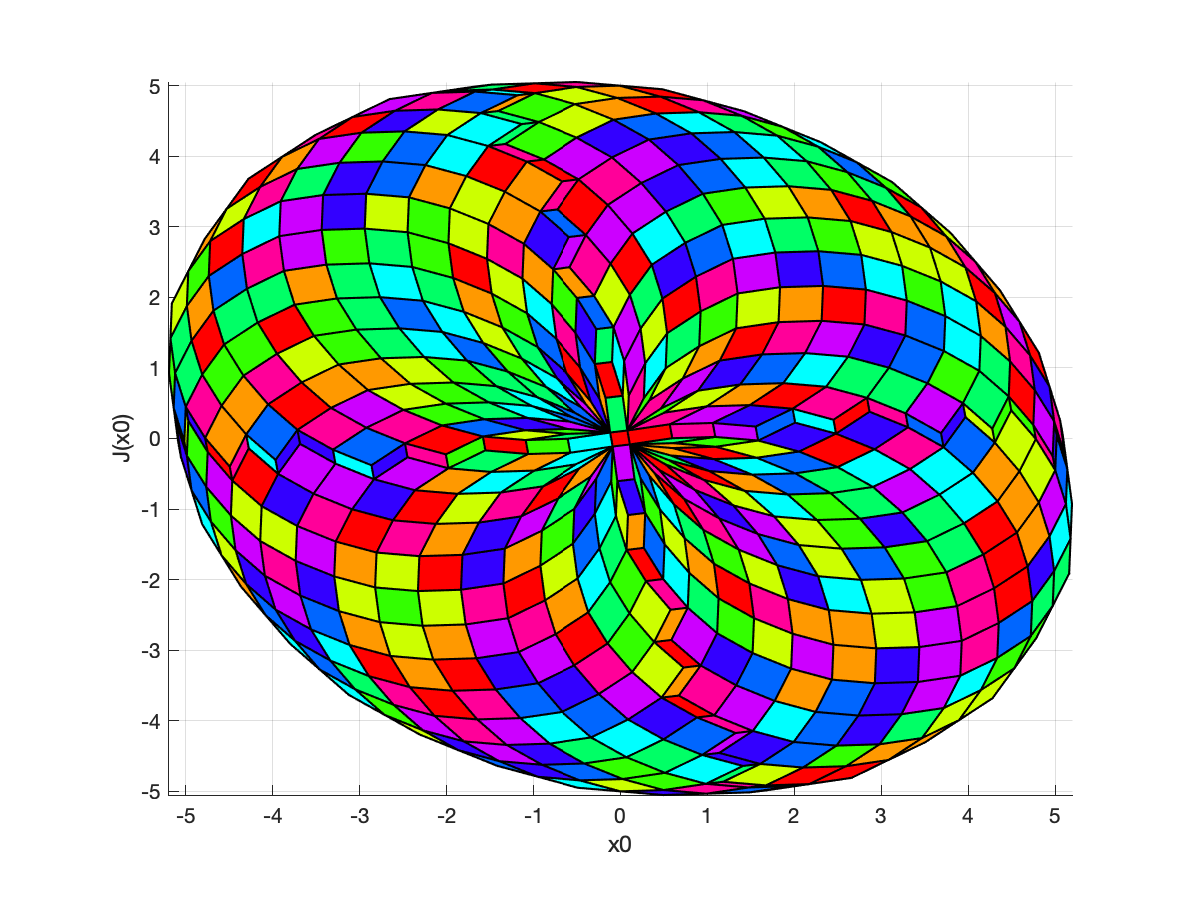
\includegraphics[width=0.8\textwidth]{figure5.eps}\\
N = 10
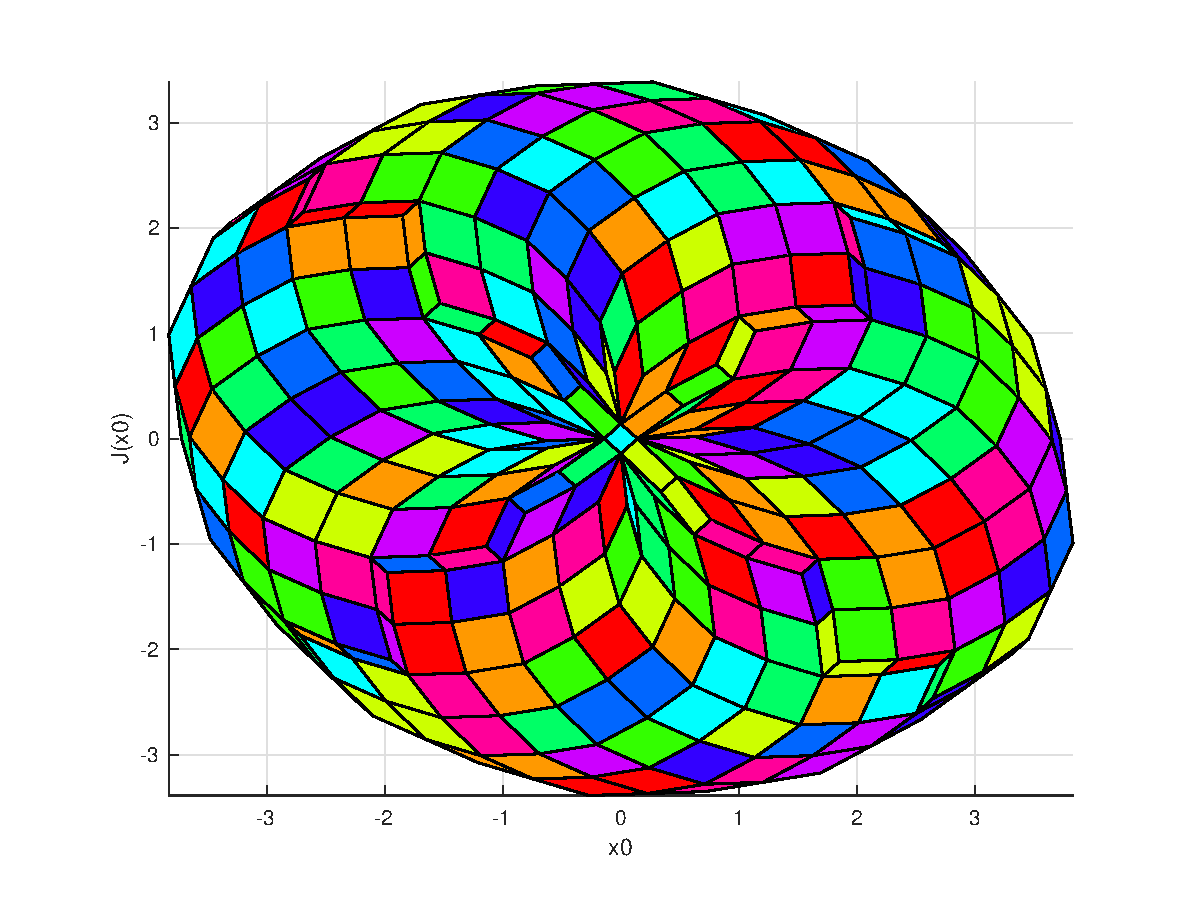
\includegraphics[width=0.8\textwidth]{figure10.eps}\\
N = 5
\includegraphics[width=0.8\textwidth]{figure15.eps}\\
N = 1
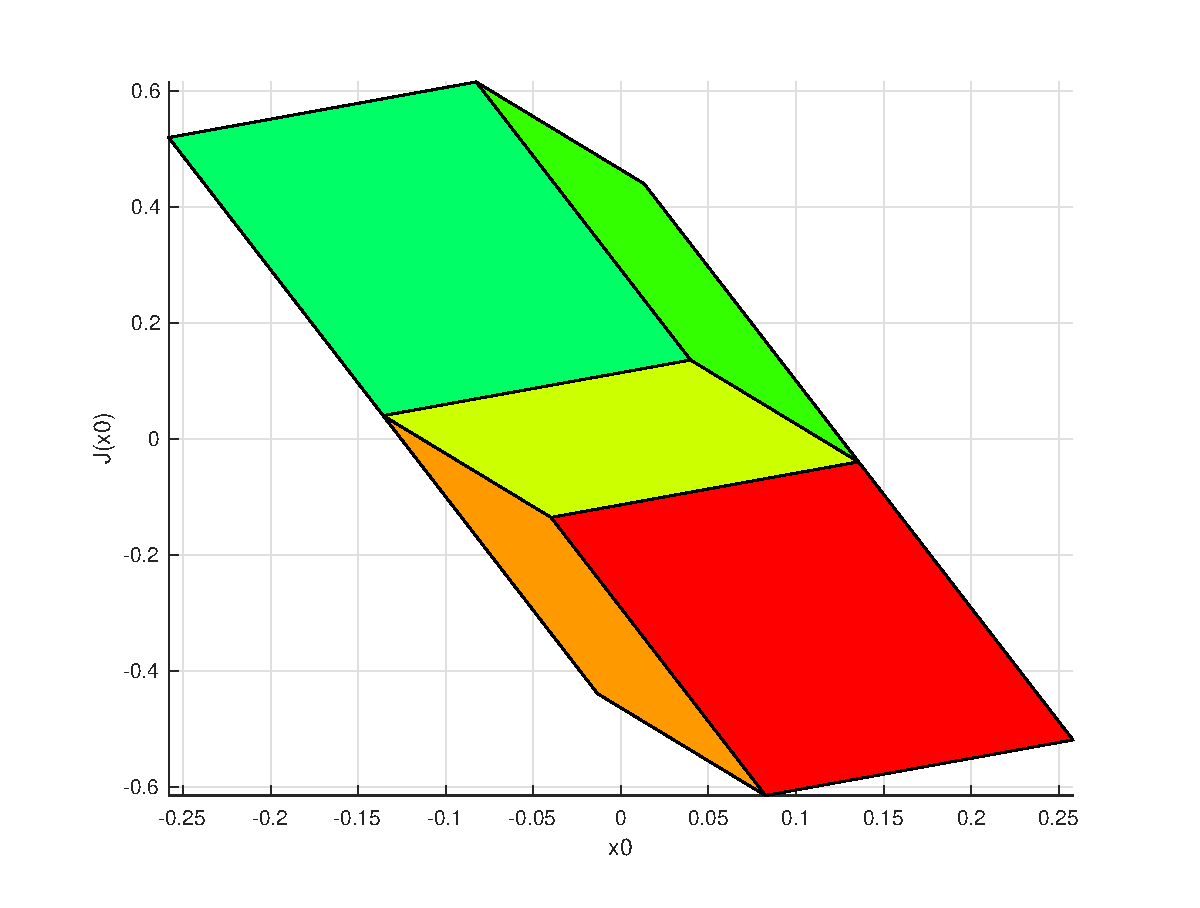
\includegraphics[width=0.8\textwidth]{figure20.eps}\\
X и U
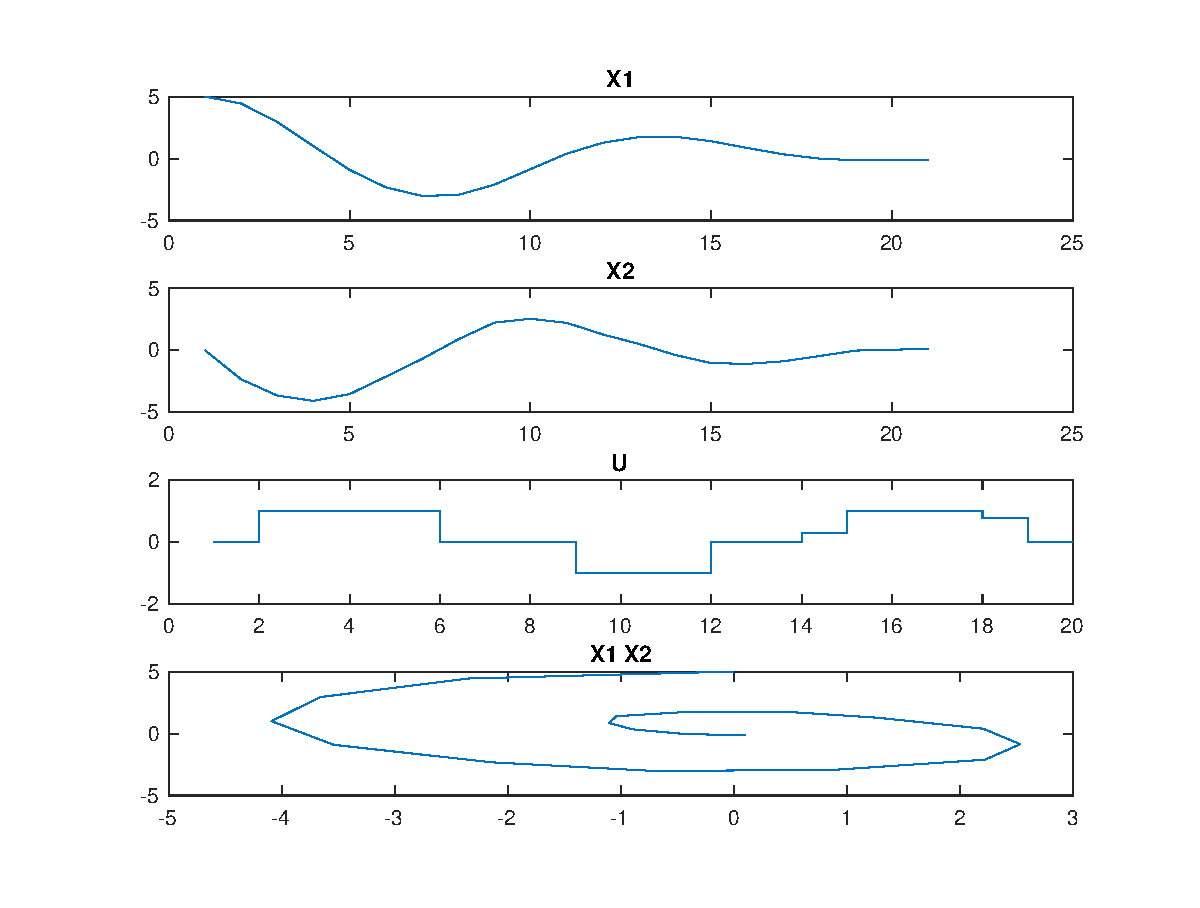
\includegraphics[width=0.8\textwidth]{graphics.eps}